
\addcontentsline{toc}{section}{Appendix} % Remove this if you don't want the appendix included in the table of contents.
\appendix

\section{MATLAB Code} \label{sec:matlab_code}
\subsection{Initialization code for Part I and Part II}
\begin{lstlisting}[caption={Matlab code showing initialization of constants used in the assignment},label={lst:p1p2},language=Matlab]
    %%%%%%%%%%% Physical constants
    g = 9.81; % gravitational constant [m/s^2]
    l_c = 0.46; % distance elevation axis to counterweight [m]
    l_h = 0.66; % distance elevation axis to helicopter head [m]
    l_p = 0.175; % distance pitch axis to motor [m]
    m_c = 1.92; % Counterweight mass [kg]
    m_p = 0.72; % Motor mass [kg]

    L_2 = (l_c*m_c-2*l_h*m_p)*g;
    K_f = - (L_2)/(l_h *6.75);  % Calculated from problem 5.1.4

    L_1 = l_p*K_f;
    L_3 = l_h*K_f;
    L_4 = -K_f*l_h;

    Vs_star = -(L_2/L_3);

    K_1 = K_f / (2*m_p*l_p);
    K_2 = (l_h*K_f) / (m_c*l_c^2 + 2*m_p*l_h^2);
    K_3 = (K_f*l_h*g*(l_c*m_c-2*l_h*m_p))
        /(l_h*K_f*(m_c*l_c^2 + 2*m_p*(l_h^2 + l_p^2)));
    K_pd = 9; %Gain for derivative part of PD
    K_pp = 0.25*K_1*K_pd^2; % xi = 1 for critical damped system

    K_rp = -1; % Gain for P regulator in travel controller
\end{lstlisting}


\subsection{Part III}
\medskip

\begin{lstlisting}[caption={Matlab code showing the calculation of the controllability matrix },label={lst:p3p2},language=Matlab]
    A3_2 = [0 1 0;  0 0 0;  0 0 0];
    B3_2 = [0 0;    0 K_1;  K_2 0];
    C3_2 = [1 0 0;   0 0 1];

    Q3_2 = diag([150 10 250]);
    R3_2 = diag([1 1]);
    K3_2 = lqr(A3_2,B3_2,Q3_2,R3_2);
    P3_2 = inv(C3_2*inv(B3_2*K3_2-A3_2)*B3_2);
\end{lstlisting}

\medskip
\begin{lstlisting}[caption={MATLAB code showing implimantation of the Marix calculation fpr part 3 problem 3 },label={lst:p3p3},language=Matlab]
    A3_3 = [0 1 0 0 0;  0 0 0 0 0;  0 0 0 0 0;  1 0 0 0 0;  0 0 1 0 0];
    B3_3 = [0 0;    0 K_1;  K_2 0;  0 0;    0 0];
    C3_3 = [C3_2, zeros(2)];
    F3_3 = [0 0;    0 0;    0 0;    -1 0;   0 -1];

    Q3_3 = diag([150 10 250 50 140]);
    R3_3 = diag([1 1]);
    %Calculation of the K and P matrix
    K3_3 = lqr(A3_3, B3_3,Q3_3,R3_3);
    P3_3 = inv(C3_2*inv(B3_2*K3_3(:,1:3)-A3_2)*B3_2);
\end{lstlisting}

\bigskip
\subsection{Part IV}

\begin{lstlisting}[caption={Matlab code showing the calculation of the controllability matrix },label={lst:p4p3},language=Matlab]
    % The C-matrix for the output y=[~e,~lambda]
    C4_3 = [0 0 1 0 0 0;    0 0 0 0 1 0];
    % The C-matrix for the output y=[~p,~e]
    C4_3p = [1 0 0 0 0 0;   0 0 1 0 0 0];
    
    % observability  
    C4= obsv(A4_2, C4_3); 
    a = rank(C4);           %gives rank at 6
    C5 = obsv(A4_2, C4_3p); 
    b = rank(C5);           %give rank equal 4
\end{lstlisting}







\newpage
\section{Simulink Diagram} \label{sec:simulink_diagrams} %%%%%%%%%%%%%%%%%%%%%%%%%%%%%%%%%%%%%%%%%%%%%%%%%%%%%%%%%%%%%%%%%%%%%%%%%%%%%%%%%%%%%%%%%%%%%%%%%%%%%%%%%%%%%%%%%%%%%%
\subsection{Part I}
\begin{figure}[H]\label{sim:part1}
    \begin{center}
    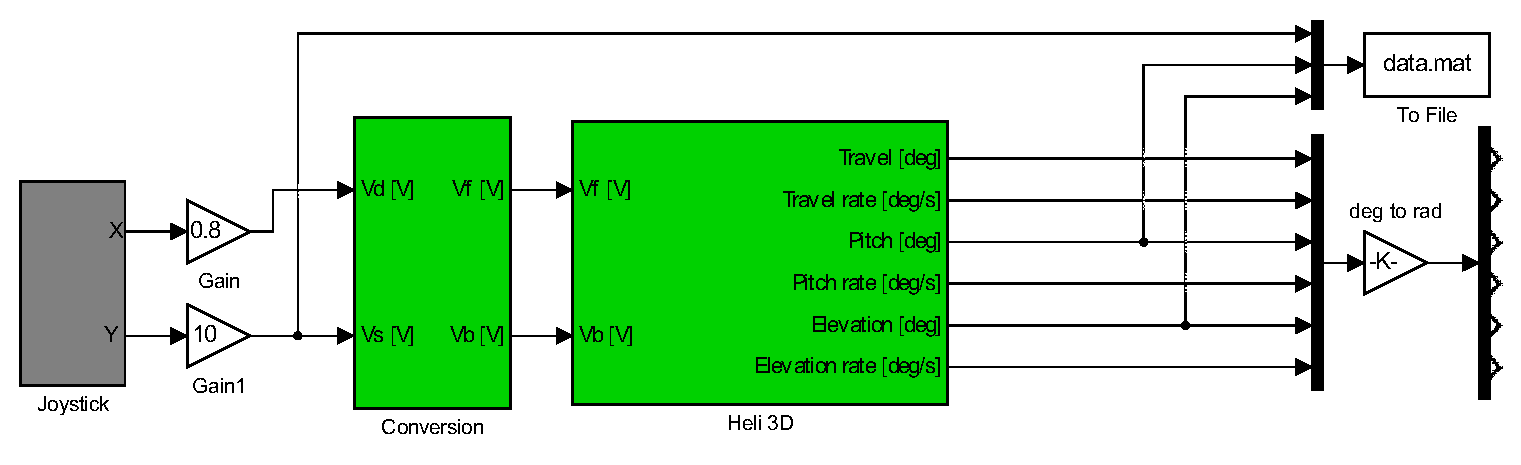
\includegraphics[width=1\linewidth]{Part1_Pictures/p1p4sys.eps}
    \caption{System for Part I}
    \end{center}
\end{figure}

\begin{figure}[H]
\begin{subfigure}{0.5\textwidth}
    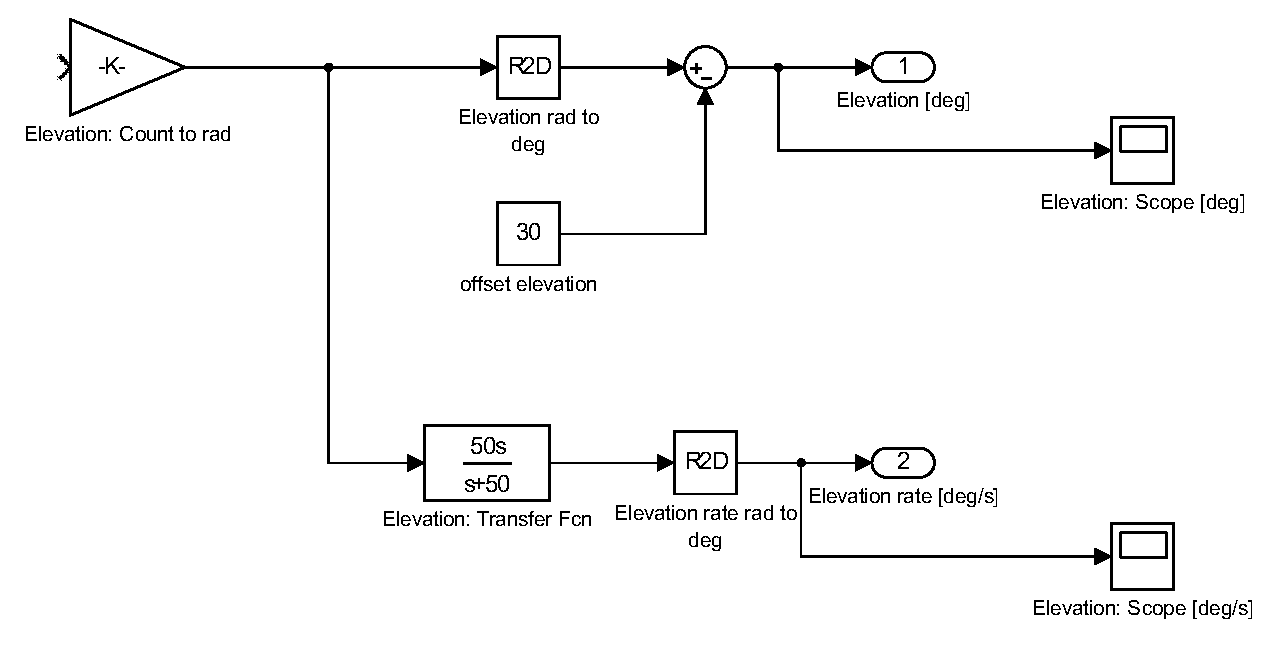
\includegraphics[width=0.9\linewidth]{Part1_Pictures/p1p4offset.eps} 
\end{subfigure}
\begin{subfigure}{0.5\textwidth}
    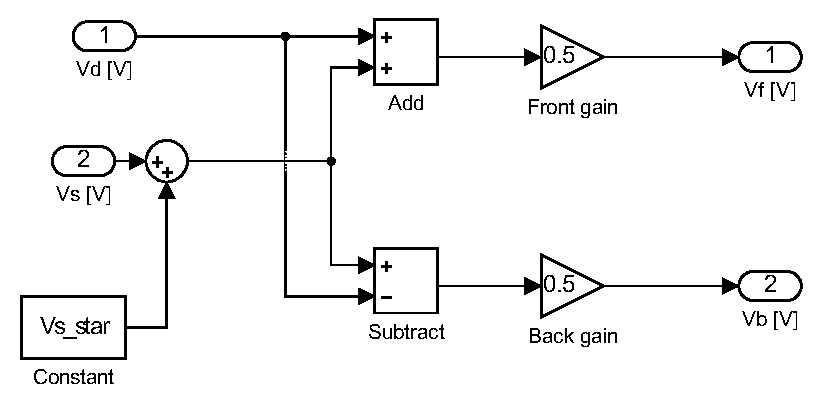
\includegraphics[width=0.9\linewidth]{Part2_pictures/p2p1_Vs_added.eps}
\end{subfigure}
\caption{Offset added in the Heli 3D block, $V_s*$ added in Conversion block}
\label{fig:vs_add}
\end{figure}


\subsection{Part II}
\begin{figure}[H]
    \begin{center}
    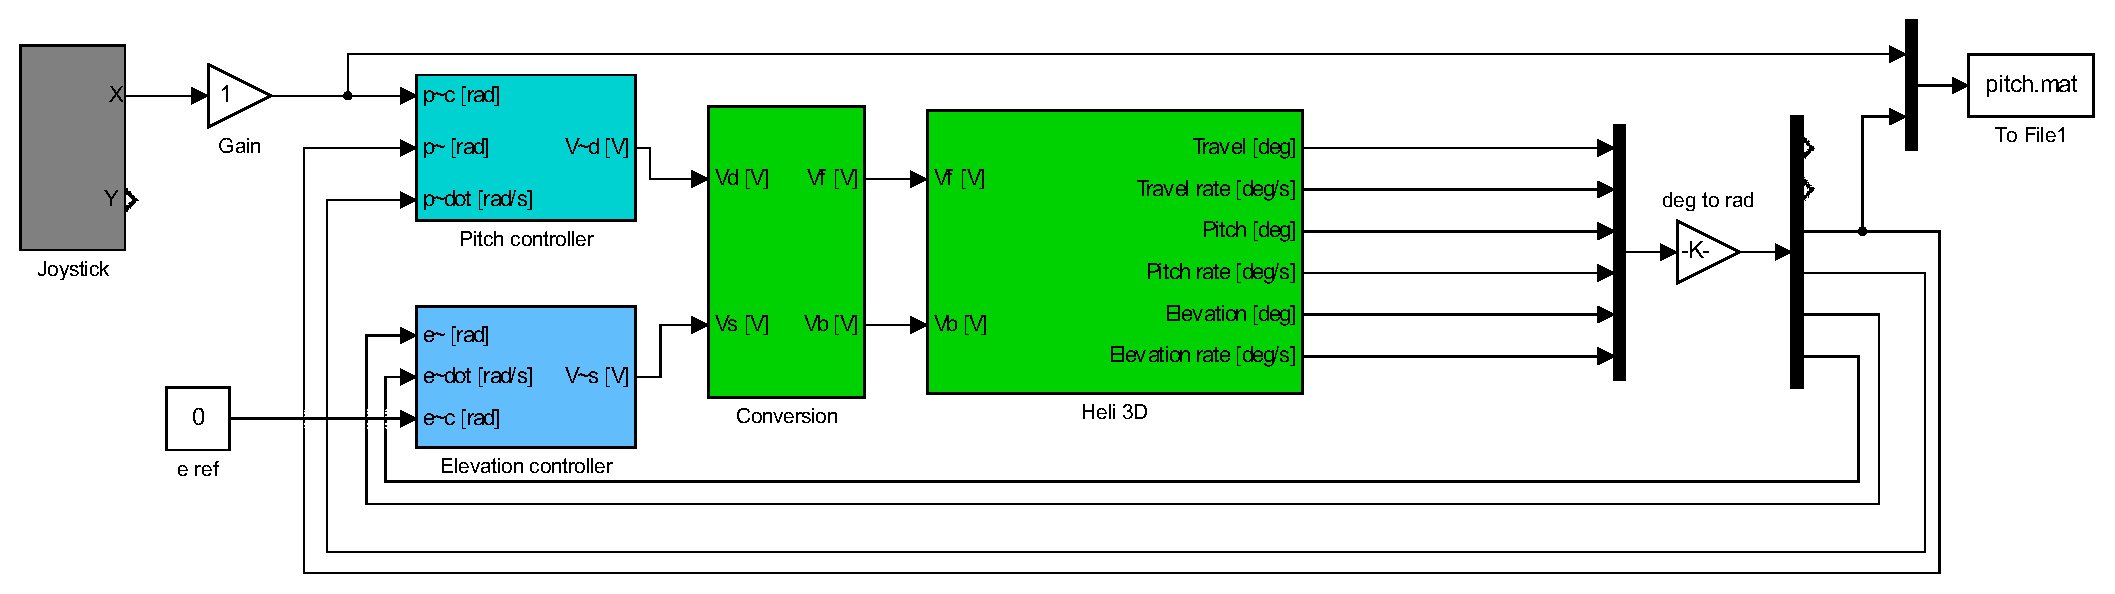
\includegraphics[width=1\linewidth]{Part2_pictures/p2p1sys.eps}
    \caption{System for problem 1}
    \end{center}
\end{figure}

\begin{figure}[H]
    \begin{center}
    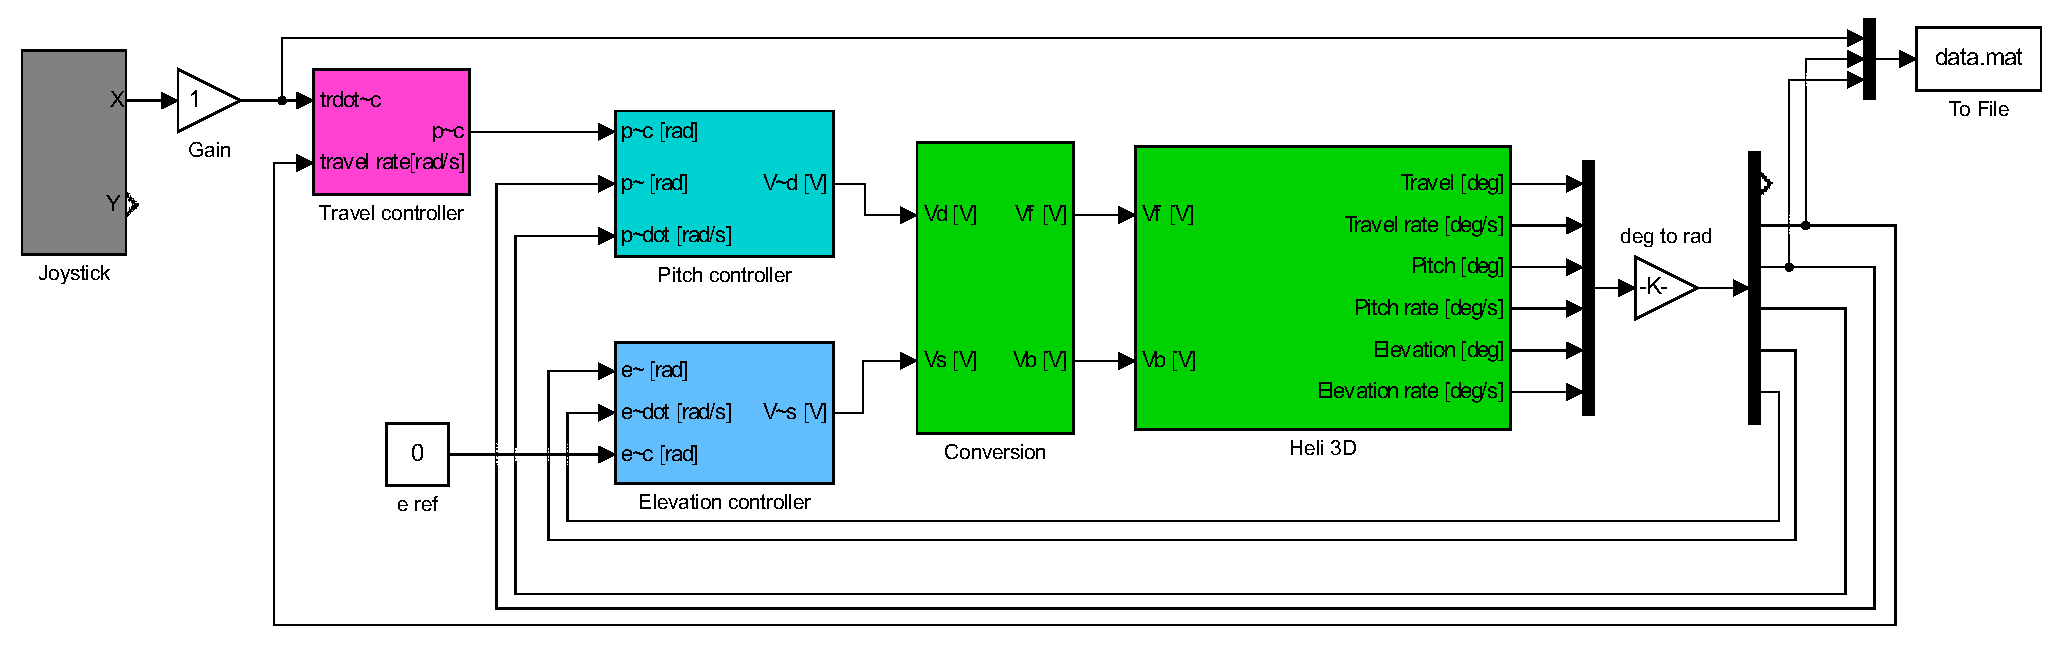
\includegraphics[width=1\linewidth]{Part2_pictures/p2p2sys.eps}
    \caption{System for problem 2}
    \end{center}
\end{figure}

\begin{figure}[H]
\begin{subfigure}{0.5\textwidth}
    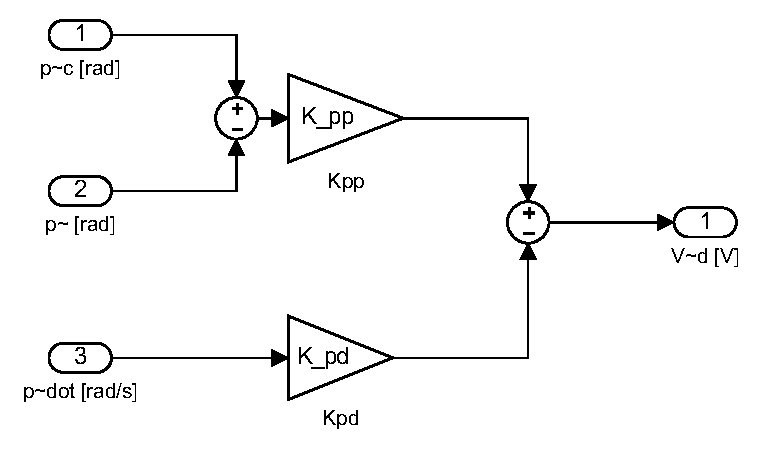
\includegraphics[width=0.9\linewidth]{Part2_pictures/p2p1_pd.eps} 
\end{subfigure}
\begin{subfigure}{0.5\textwidth}
    \includegraphics[width=0.9\linewidth]{Part2_pictures/p2p2_p.eps}
\end{subfigure}
\caption{Pitch controller block and Travel controller block}
\end{figure}

\subsection{Part III}
\begin{figure}[H]
    \begin{center}
    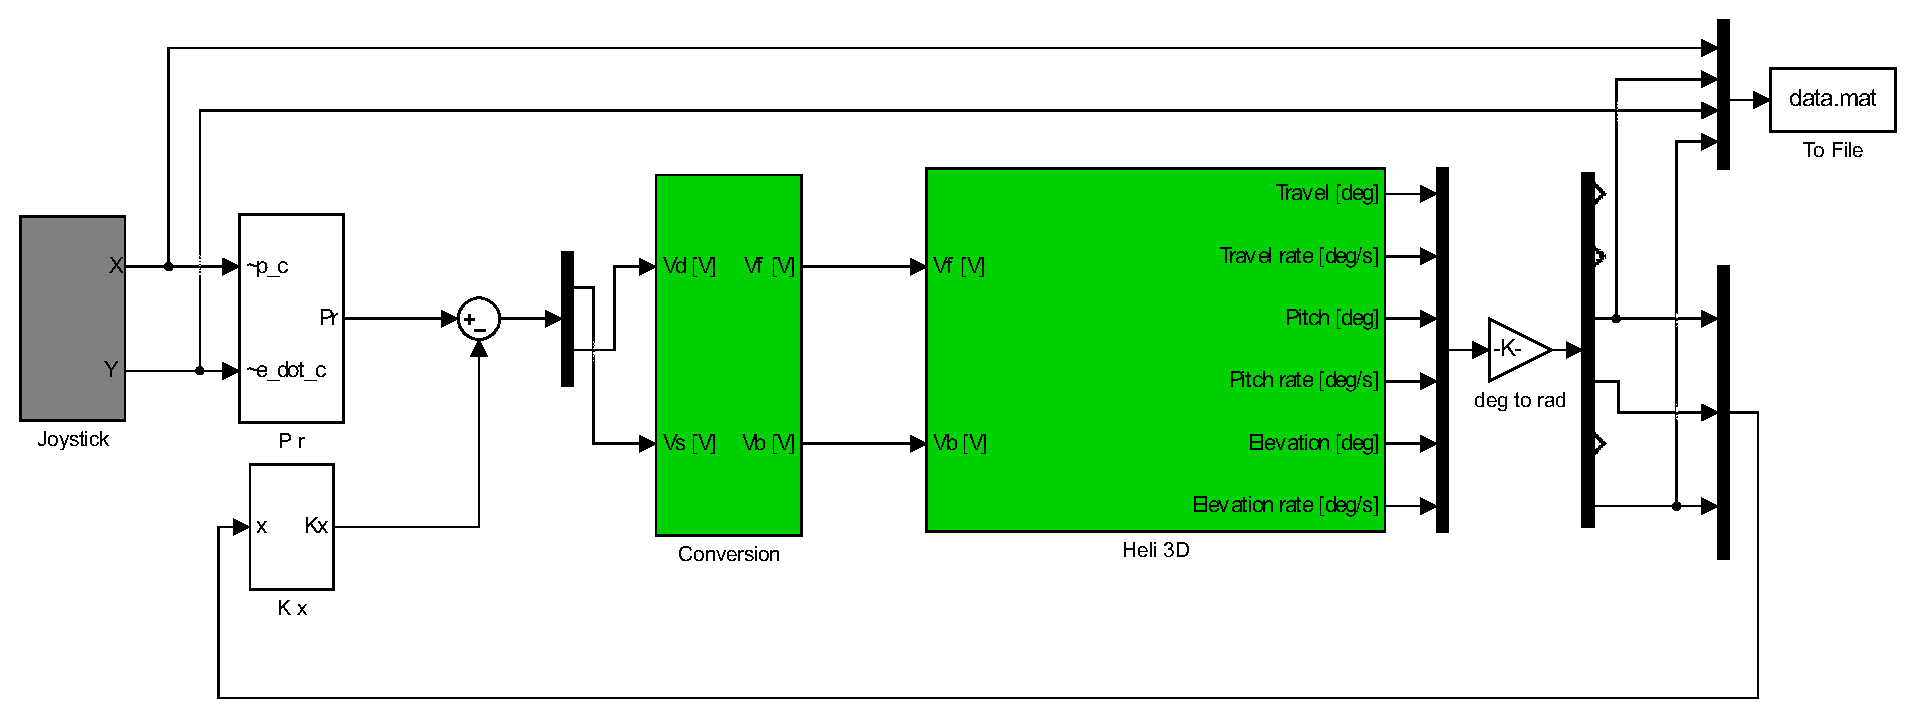
\includegraphics[width=1\linewidth]{Part3_pictures/p3p2sys.eps}
    \caption{System for problem 2}
    \label{sim:u=p3p2}
    \end{center}
\end{figure}

\begin{figure}[H]
    \begin{center}
    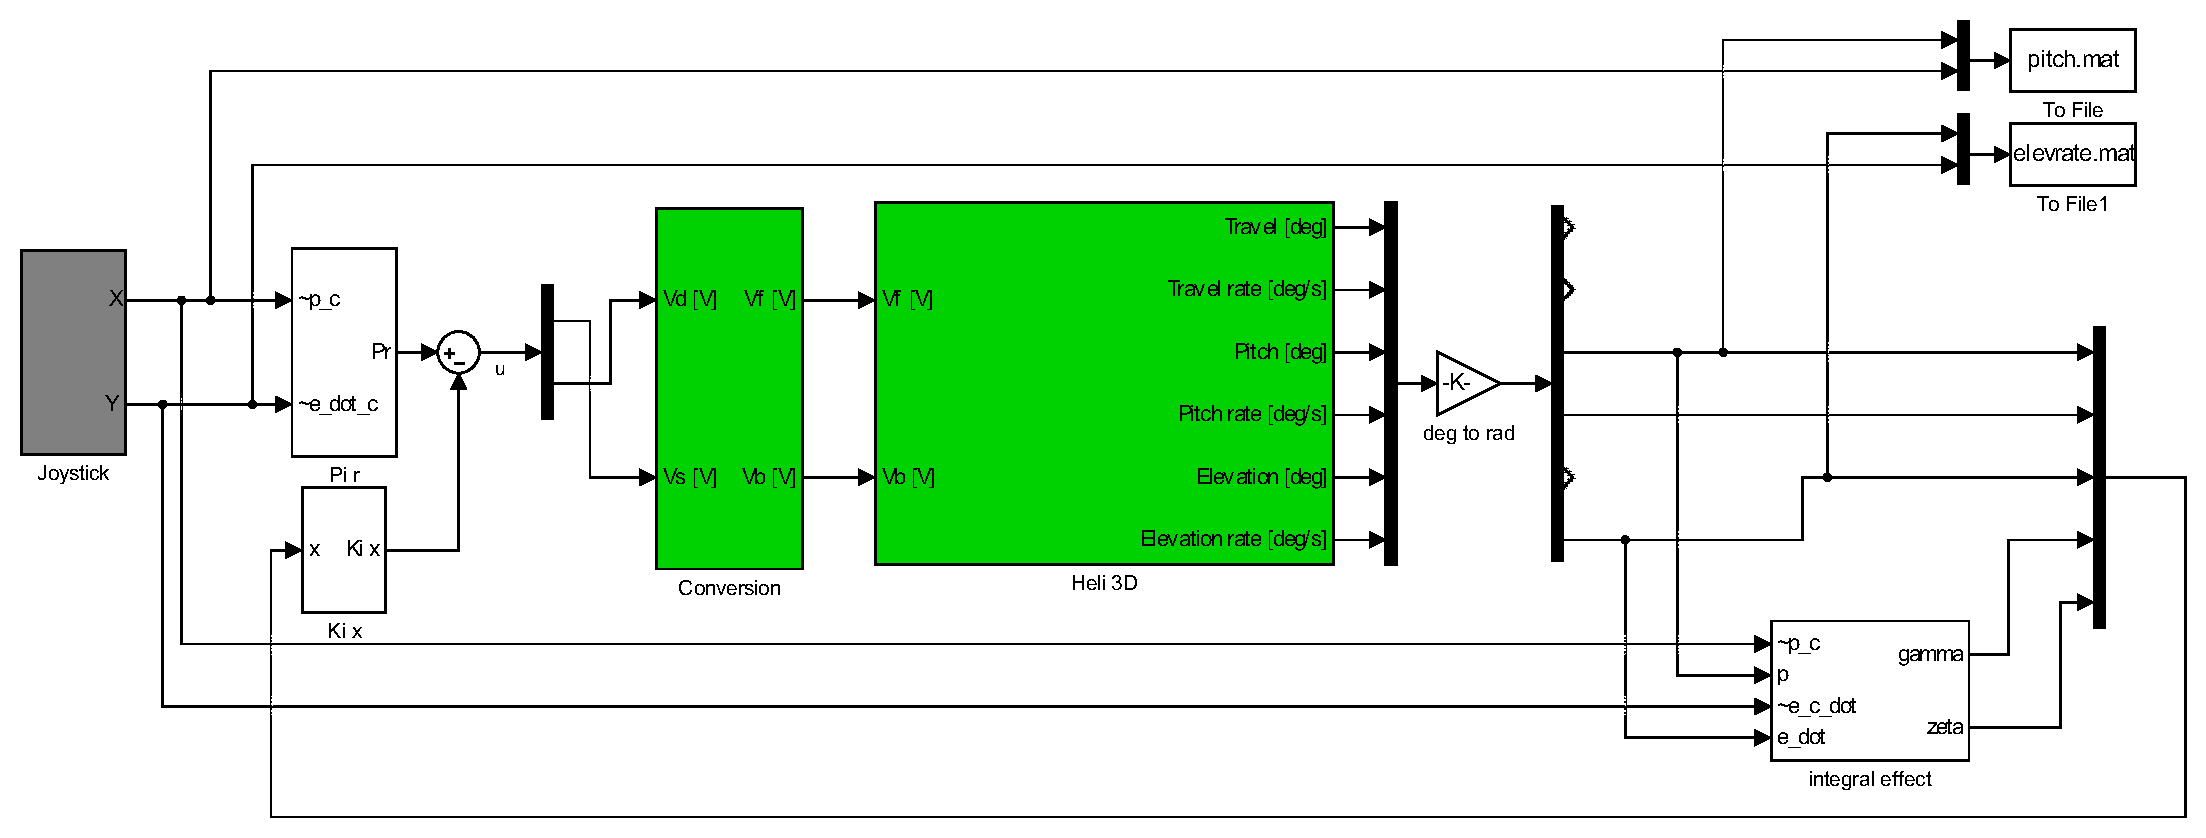
\includegraphics[width=1\linewidth]{Part3_pictures/p3p3sys.eps}
    \caption{System for problem 3}
    \end{center}
\end{figure}

\begin{figure}[H]
\graphicspath{ {Part3_pictures/}}
\begin{subfigure}{0.5\textwidth}
    \includegraphics[width=0.9\linewidth]{Part3_pictures/p3p2_Pr.eps} 
\end{subfigure}
\begin{subfigure}{0.5\textwidth}
    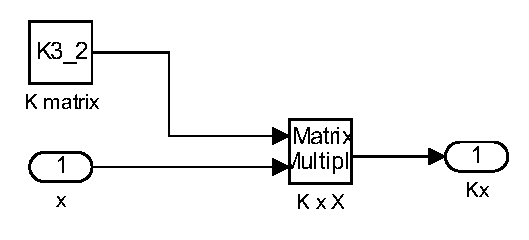
\includegraphics[width=0.9\linewidth]{Part3_pictures/p3p2_Kx.eps}
\end{subfigure}
\caption{Pr and Kx blocks (in Pi r and Ki x the only difference is $P3\_2 = P3\_3$ and $K3\_2 = K3\_3$)}
\end{figure}

\begin{figure}[H]
    \begin{center}
    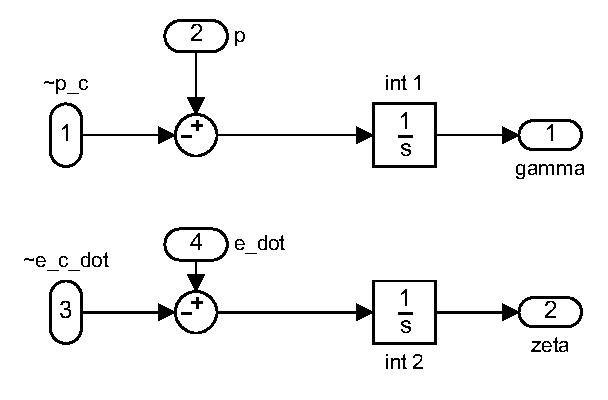
\includegraphics[width=0.5\linewidth]{Part3_pictures/p3p3_int.eps}
    \caption{Integral effect block}
    \end{center}
\end{figure}

\subsection{Part IV}

\begin{figure}[H]
    \begin{center}
        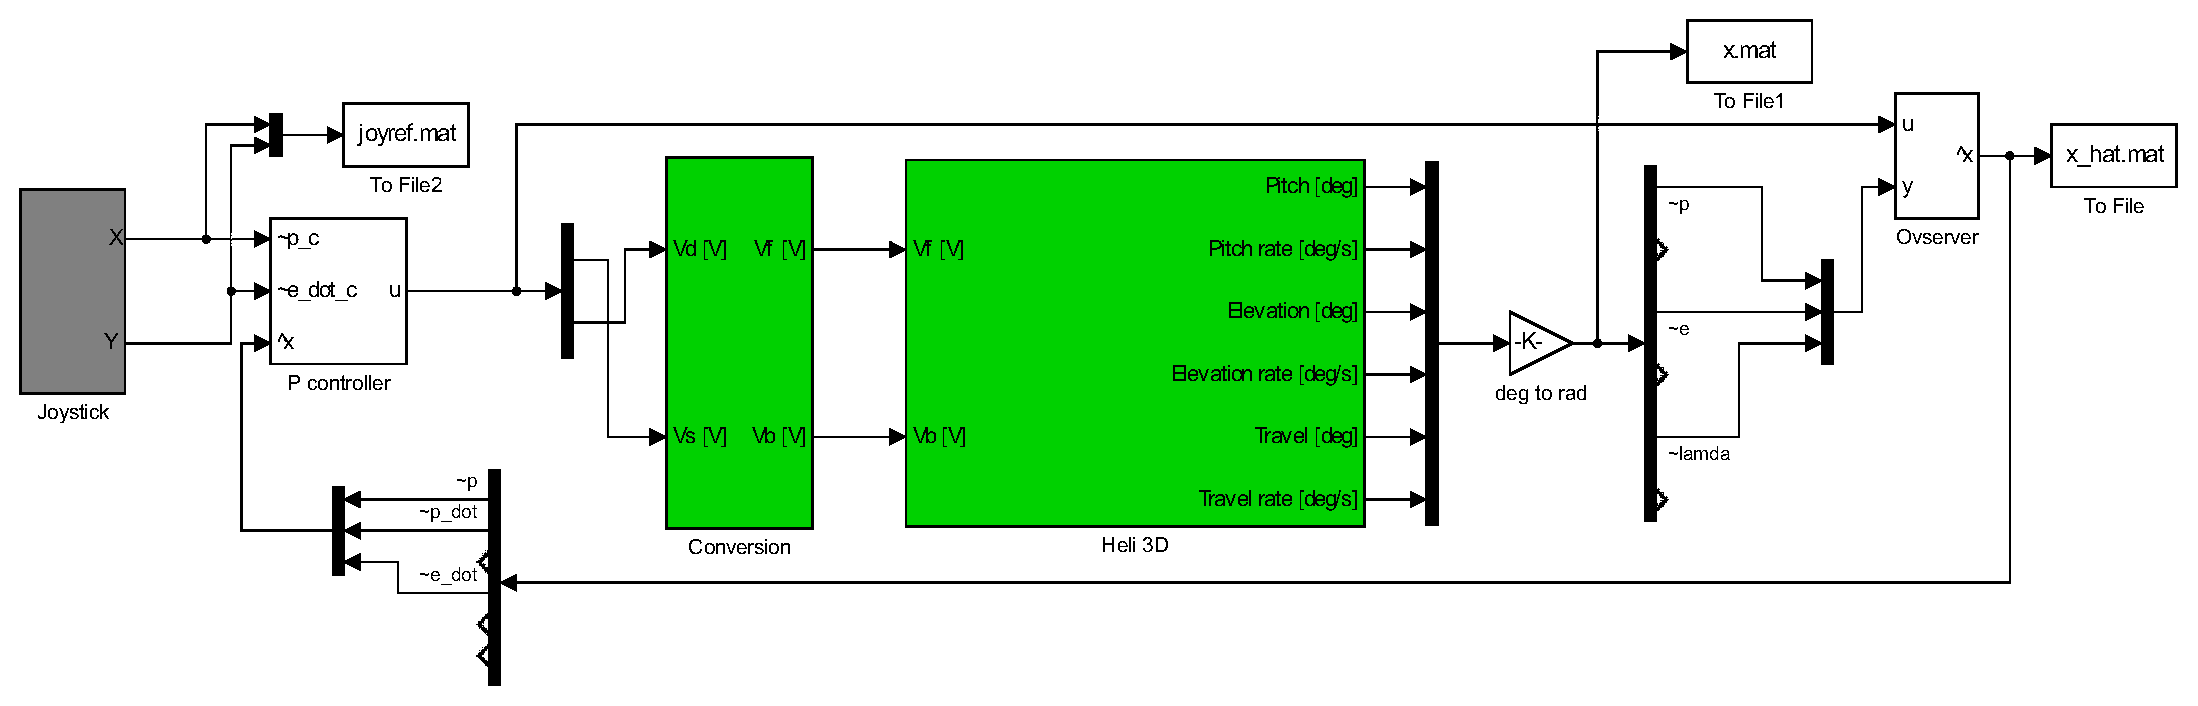
\includegraphics[width=1\linewidth]{Part4_pictures/simulink/p4p2sys.eps} 
        \caption{System for problem 2 without integral effect}
        \label{p4p2noint}
    \end{center}
\end{figure}

\begin{figure}[H]
    \begin{center}
        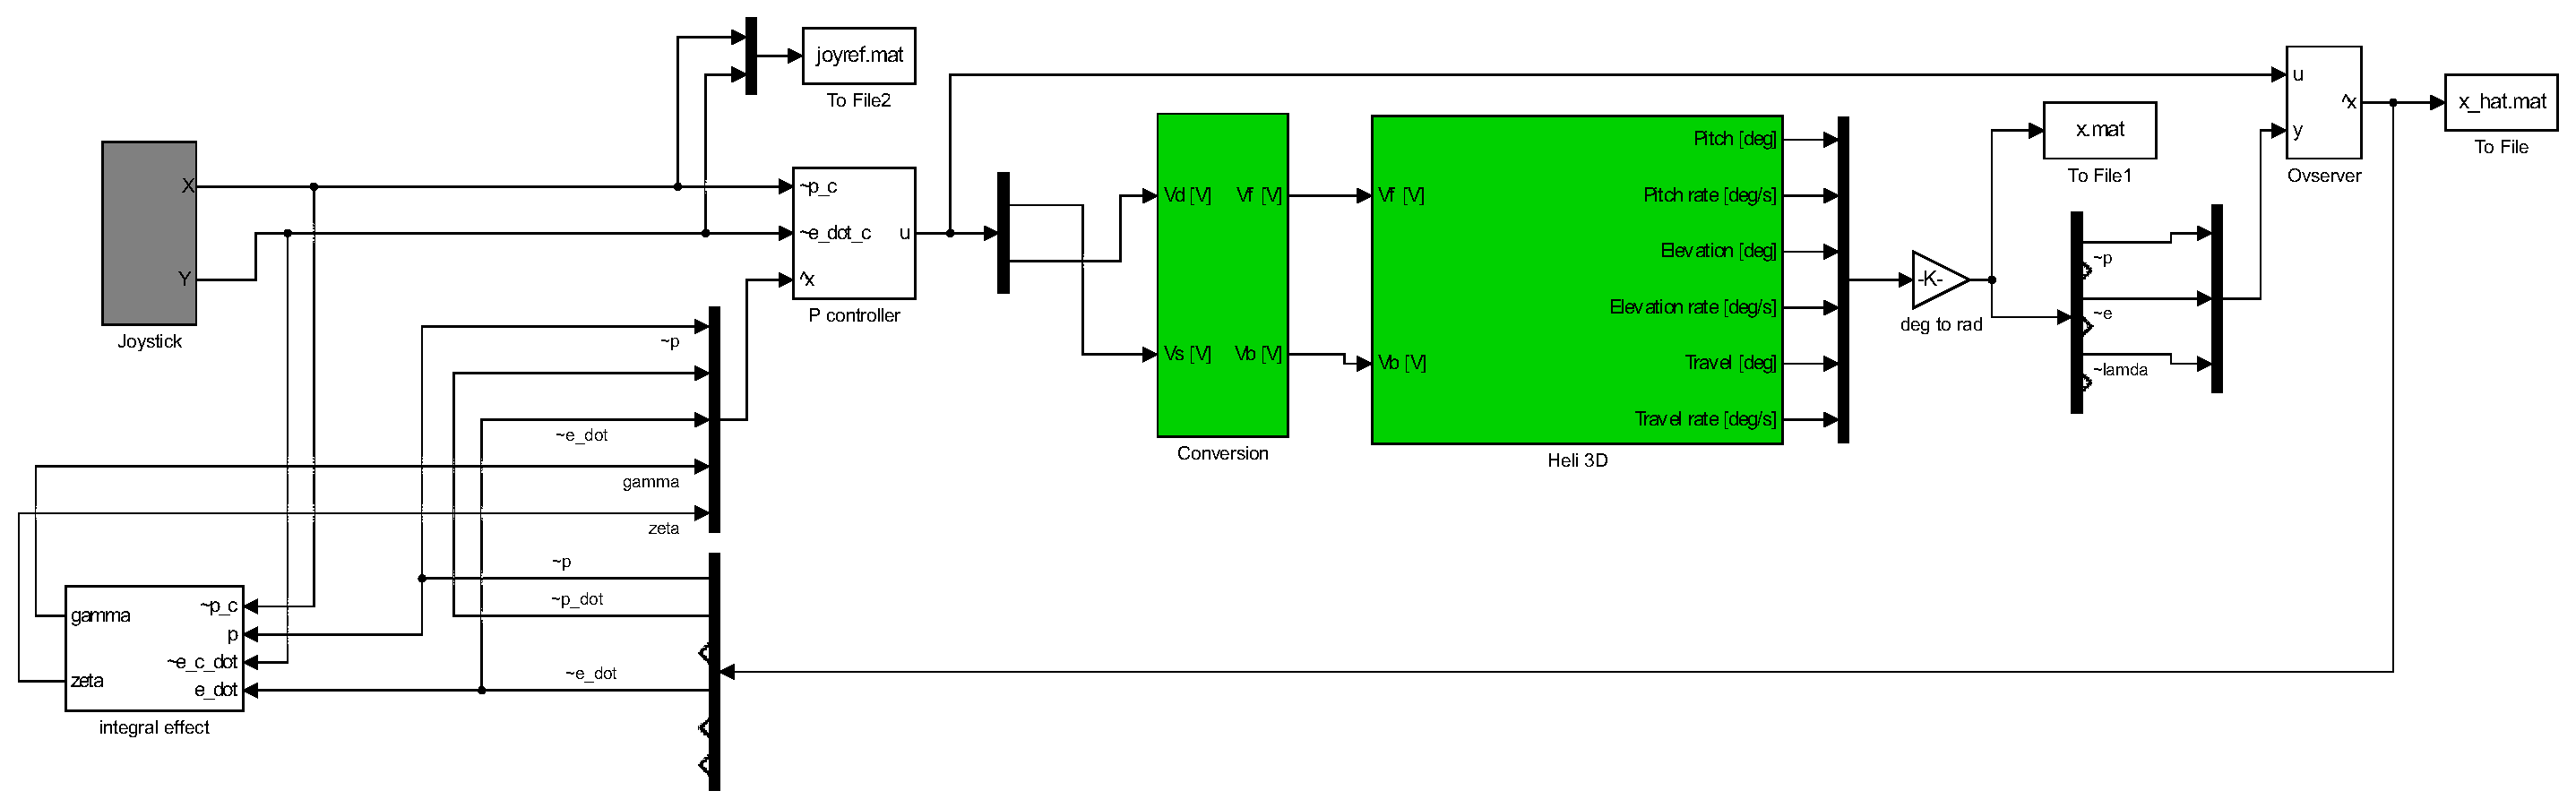
\includegraphics[width=1\linewidth]{Part4_pictures/simulink/p4p2sys_int.eps} 
        \caption{System for problem 2 with integral effect}
        \label{p4p2int}
    \end{center}
\end{figure}

\begin{figure}[H]
    \begin{center}
        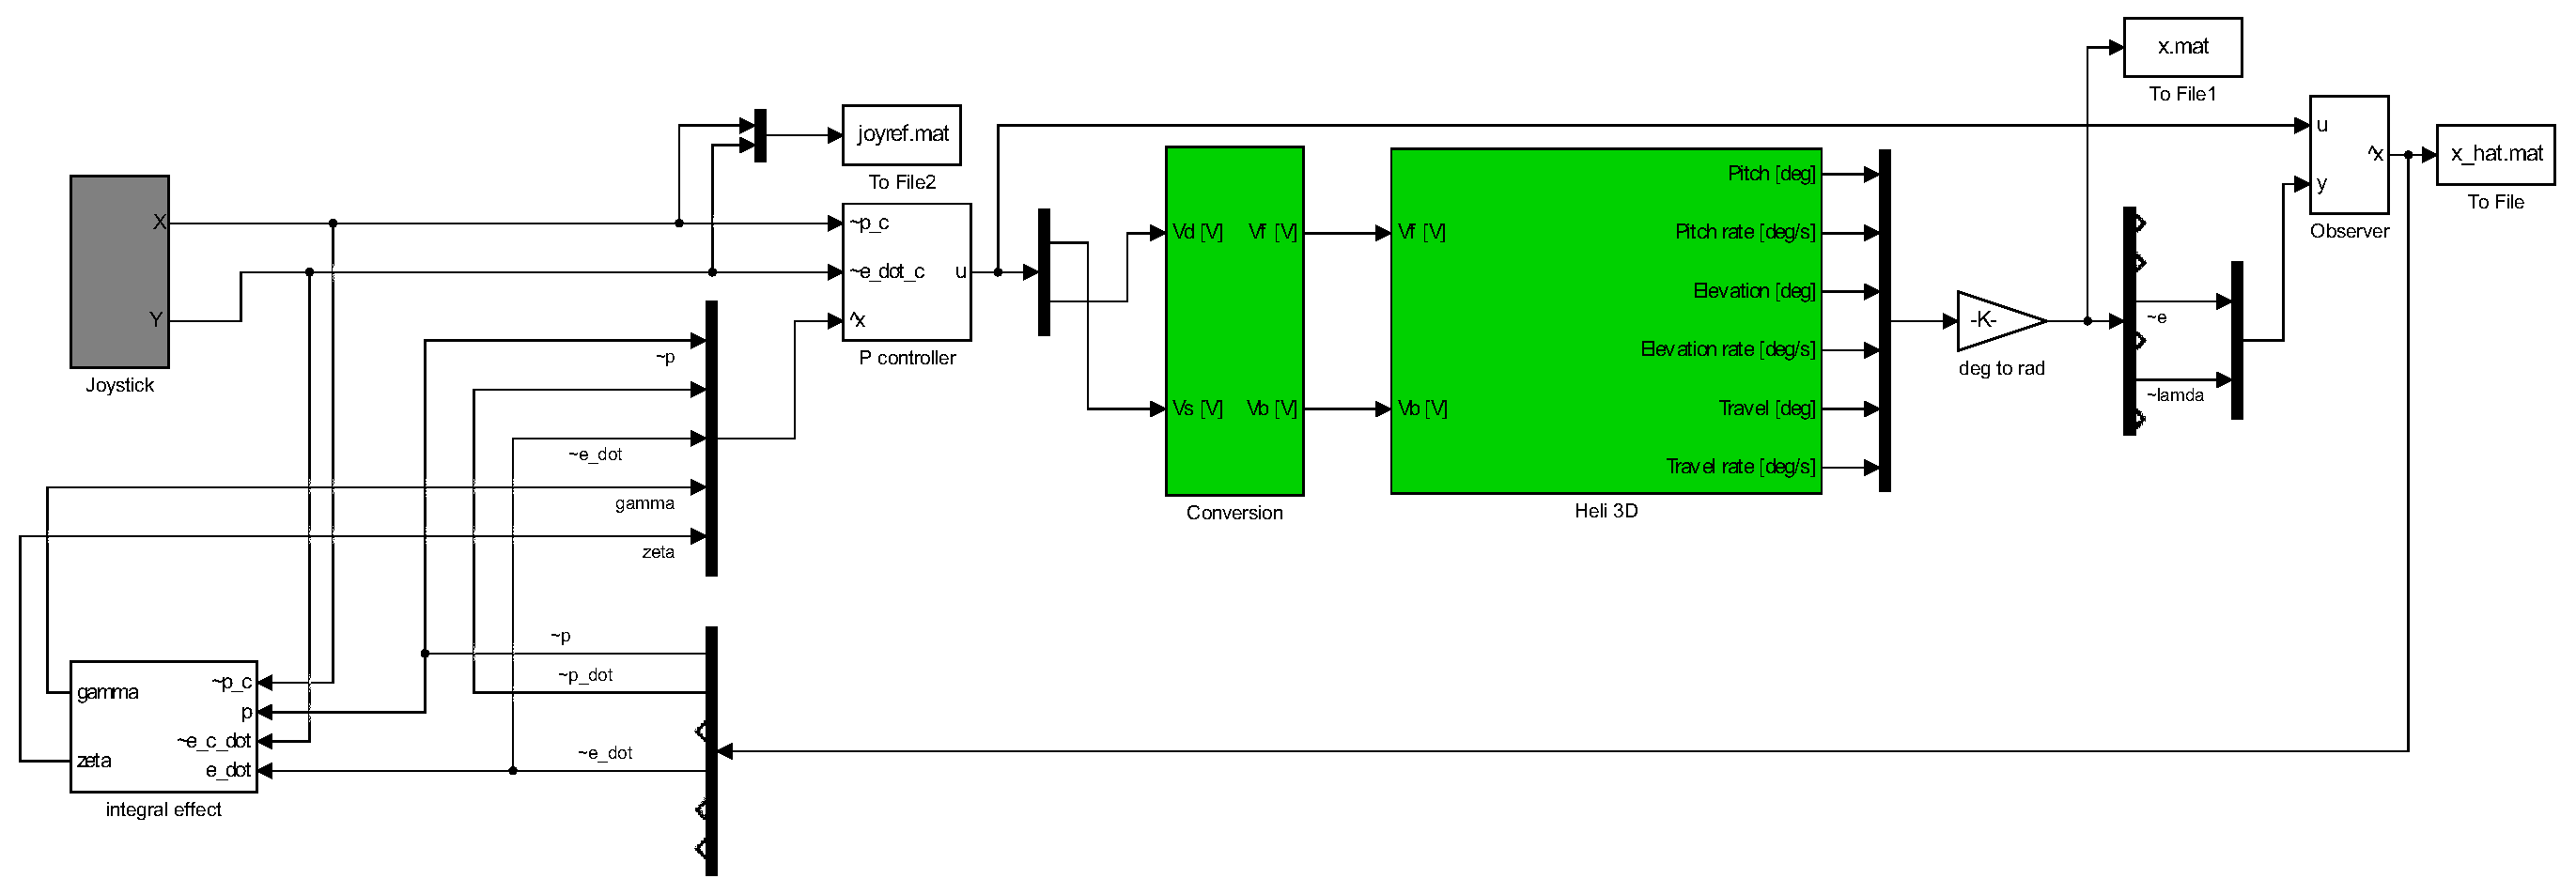
\includegraphics[width=1\linewidth]{Part4_pictures/simulink/p4p3sys.eps} 
        \caption{System for problem 3}
        \label{p4p3}
    \end{center}
\end{figure}

\begin{figure}[H]
\graphicspath{ {Part4_pictures/}}
\begin{subfigure}{0.5\textwidth}
    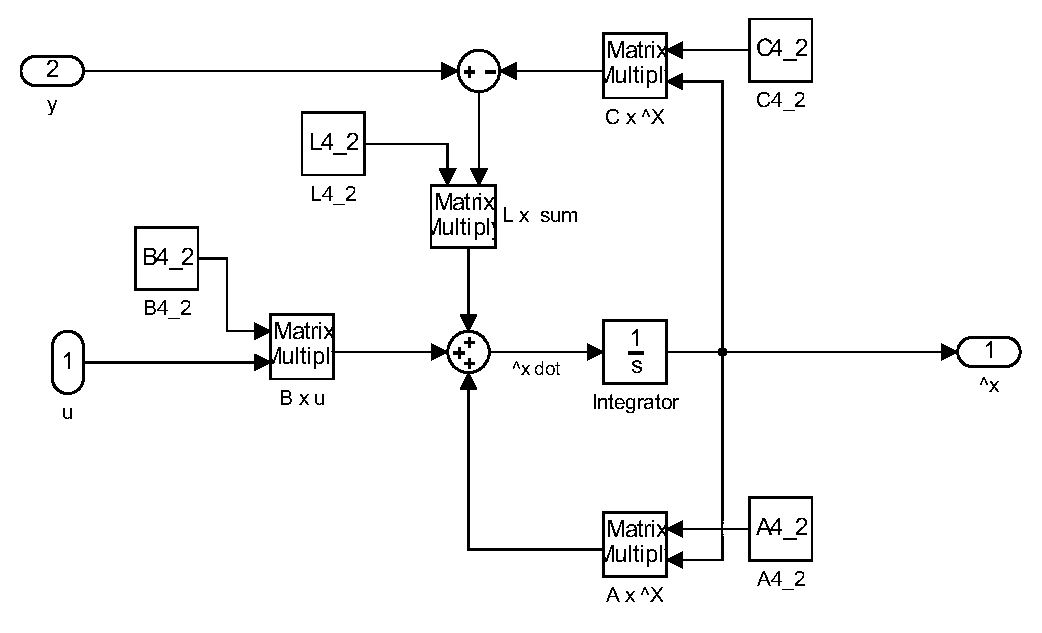
\includegraphics[width=1\linewidth]{Part4_pictures/simulink/p4p2_obs.eps} 
\end{subfigure}
\begin{subfigure}{0.5\textwidth}
    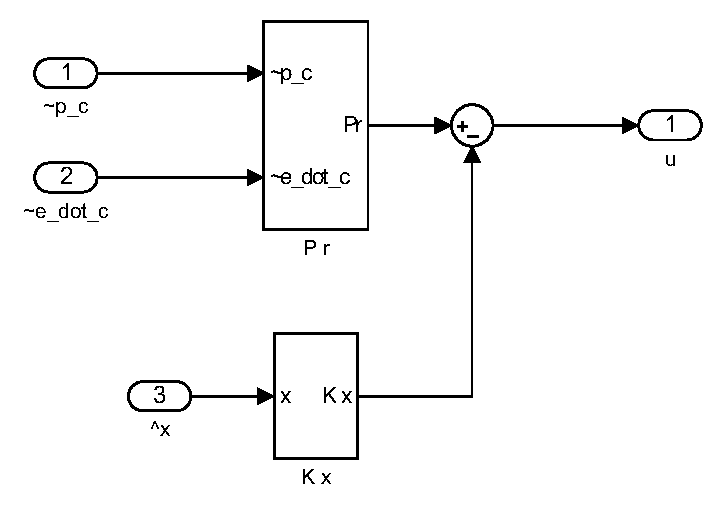
\includegraphics[width=0.9\linewidth]{Part4_pictures/simulink/p4p2_p.eps}
\end{subfigure}
\caption{Observer and P-controller blocks}
\label{p4p2_obsctr}
\end{figure}
\newpage



\section{Plots}

\subsection{Part III}
%%%%%% p3p2 bilder 
%% Forskjellige verdier av plottene 
\subsubsection{Plots with the PD controller}
\begin{figure}[H]
\graphicspath{ {Part3_pictures/}}
\begin{subfigure}{0.5\textwidth}
    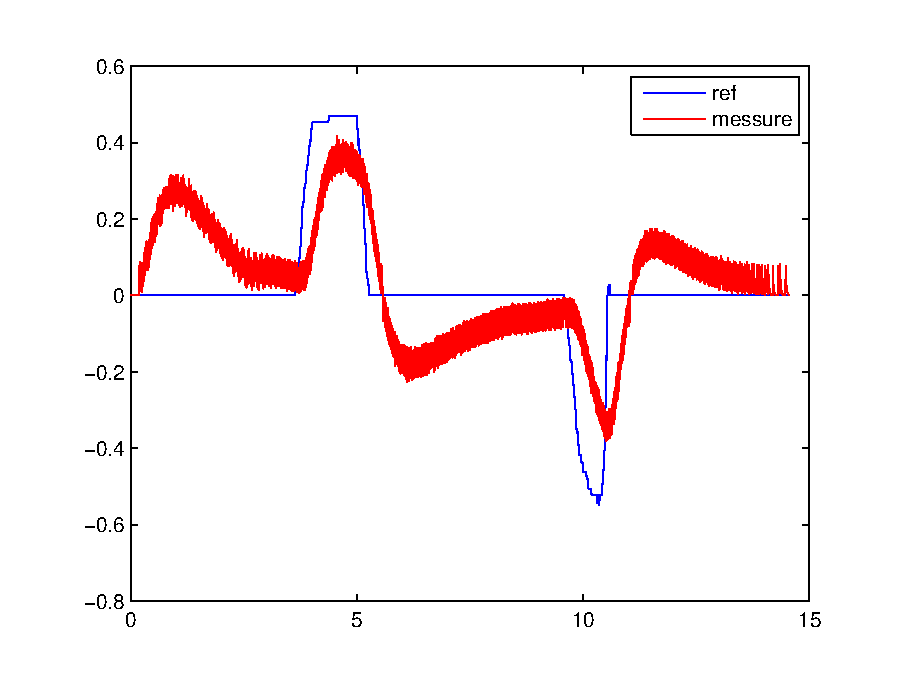
\includegraphics[width=0.9\linewidth]{Part3_pictures/p3p2/Q1elevation.eps} 
    \caption{Elevation rate}
    \label{p3p2Q1e}
\end{subfigure}
\begin{subfigure}{0.5\textwidth}
    \includegraphics[width=0.9\linewidth]{Part3_pictures/p3p2/Q1pitch.eps}
    \caption{Pitch angle}
    \label{p3p2Q1p}
\end{subfigure}
\caption{Plot with Q= [100 10 100]}
\label{p3p2Q1}
\end{figure}

\begin{figure}[H]
\graphicspath{ {Part3_pictures/}}
\begin{subfigure}{0.5\textwidth}
    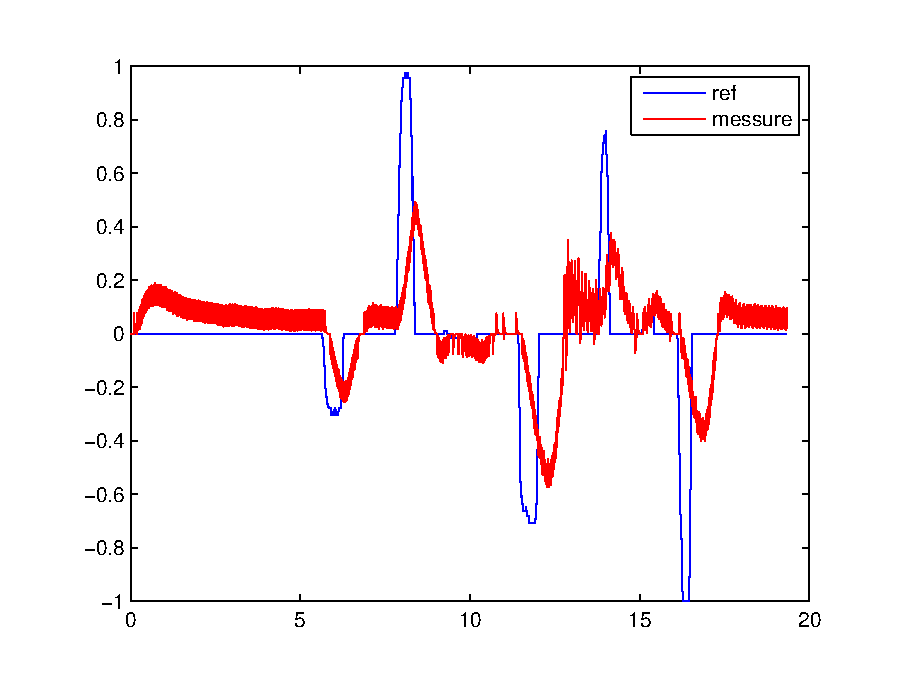
\includegraphics[width=0.9\linewidth]{Part3_pictures/p3p2/Q2elevation.eps} 
    \caption{Elevation rate}
    \label{p3p2Q2e}
\end{subfigure}
\begin{subfigure}{0.5\textwidth}
    \includegraphics[width=0.9\linewidth]{Part3_pictures/p3p2/Q2pitch.eps}
    \caption{Pitch angle}
    \label{p3p2Q2p}
\end{subfigure}
\caption{Plot with Q= [10 1 1000]}
\label{p3p2Q2}
\end{figure}

\begin{figure}[H]
\graphicspath{ {Part3_pictures/}}
\begin{subfigure}{0.5\textwidth}
    \includegraphics[width=0.9\linewidth]{Part3_pictures/p3p2/Q3elevation.eps} 
    \caption{Elevation rate}
    \label{p3p2Q3e}
\end{subfigure}
\begin{subfigure}{0.5\textwidth}
    \includegraphics[width=0.9\linewidth]{Part3_pictures/p3p2/Q3pitch.eps}
    \caption{Pitch angle}
    \label{p3p2Q3p}
\end{subfigure}
\caption{Plot with Q= [100 100 100]}
\label{p3p2Q3}
\end{figure}
\newpage

%%%%%% p3p3
%% Forskjellige verdier av plottene
\subsubsection{Plots for the PID controller}

\begin{figure}[H]
\graphicspath{ {Part3_pictures/}}
\begin{subfigure}{0.5\textwidth}
    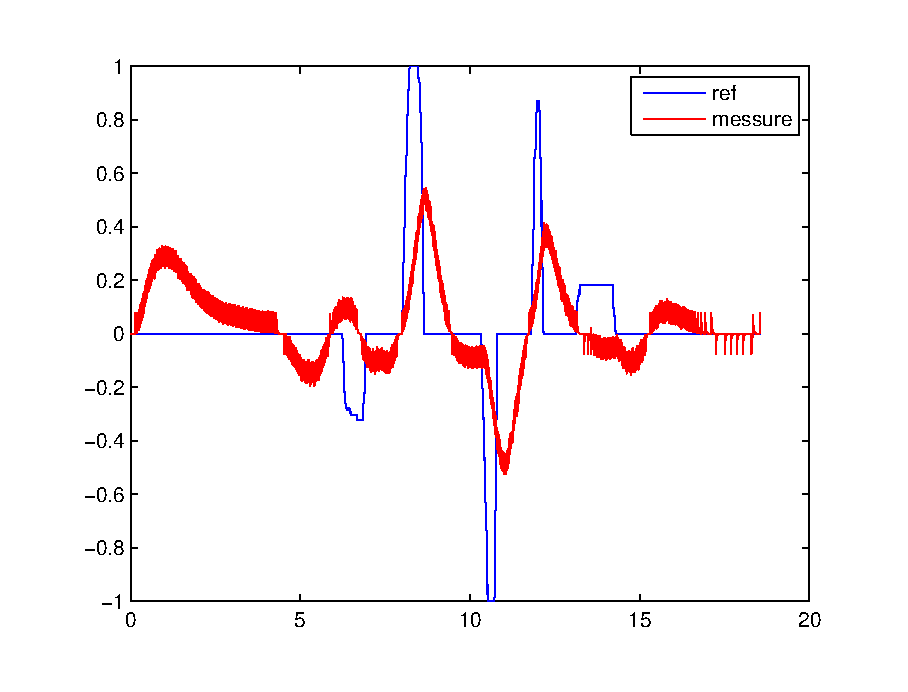
\includegraphics[width=0.9\linewidth]{Part3_pictures/p3p3/Q1elevation.eps} 
    \caption{Elevation rate}
\end{subfigure}
\begin{subfigure}{0.5\textwidth}
    \includegraphics[width=0.9\linewidth]{Part3_pictures/p3p3/Q1pitch.eps}
    \caption{Pitch angle}
\end{subfigure}
\caption{Plot with Q= [150 10 250 50 140]}
\end{figure}

\begin{figure}[H]
\graphicspath{ {Part3_pictures/}}
\begin{subfigure}{0.5\textwidth}
    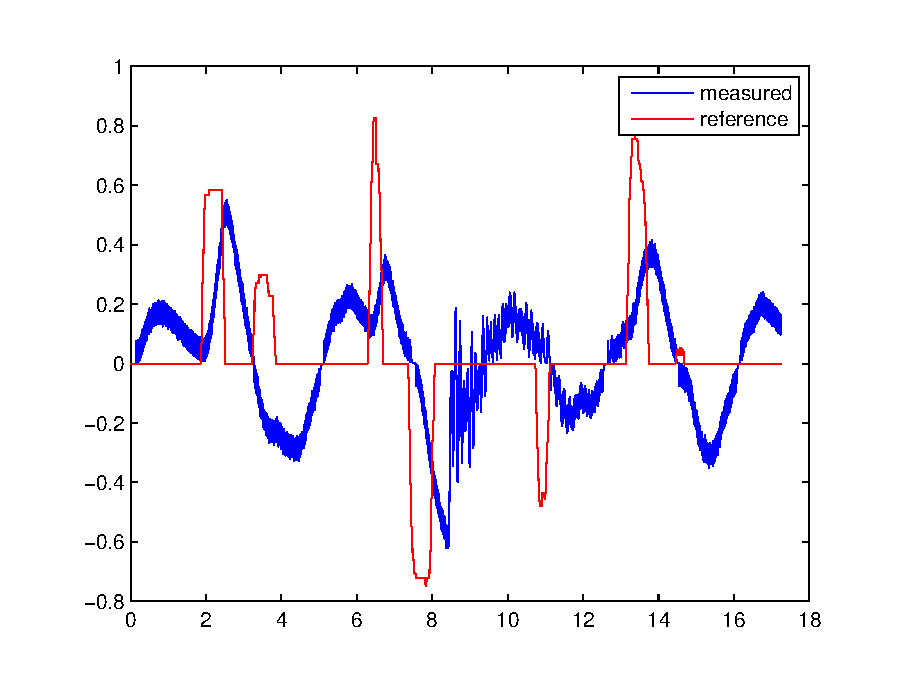
\includegraphics[width=0.9\linewidth]{Part3_pictures/p3p3/Q2elevation.eps} 
    \caption{Elevation rate}
\end{subfigure}
\begin{subfigure}{0.5\textwidth}
    \includegraphics[width=0.9\linewidth]{Part3_pictures/p3p3/Q2pitch.eps}
    \caption{Pitch angle}
\end{subfigure}
\caption{Plot with Q = [300 10 250 50 140]}
\end{figure}

\begin{figure}[H]
\graphicspath{ {Part3_pictures/}}
\begin{subfigure}{0.5\textwidth}
    \includegraphics[width=0.9\linewidth]{Part3_pictures/p3p3/Q3elevation.eps} 
    \caption{Elevation rate}
\end{subfigure}
\begin{subfigure}{0.5\textwidth}
    \includegraphics[width=0.9\linewidth]{Part3_pictures/p3p3/Q3pitch.eps}
    \caption{Pitch angle}
\end{subfigure}
\caption{Plot with Q= [75 10 250 50 140]}
\end{figure}

\begin{figure}[H]
\graphicspath{ {Part3_pictures/}}
\begin{subfigure}{0.5\textwidth}
    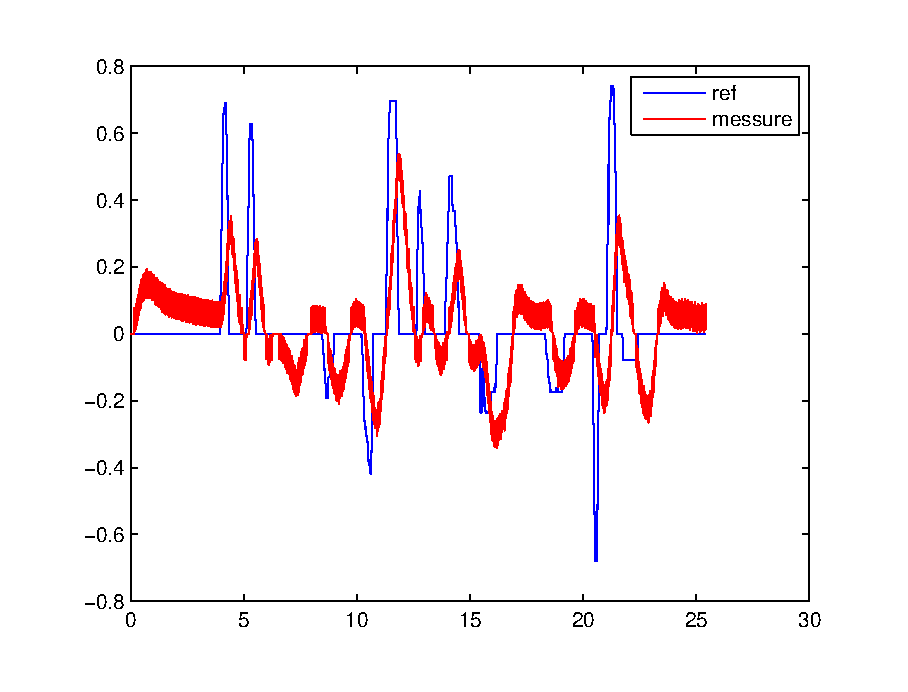
\includegraphics[width=0.9\linewidth]{Part3_pictures/p3p3/Q4elevation.eps} 
    \caption{Elevation rate}
\end{subfigure}
\begin{subfigure}{0.5\textwidth}
    \includegraphics[width=0.9\linewidth]{Part3_pictures/p3p3/Q4pitch.eps}
    \caption{Pitch angle}
\end{subfigure}
\caption{Plot with Q =[150 10 250 100 140]}
\end{figure}
\newpage



\subsection{Part IV}
\subsubsection{Without integral effect}

\begin{figure}[H]
\graphicspath{ {Part4_pictures/}}
\begin{subfigure}{0.5\textwidth}
    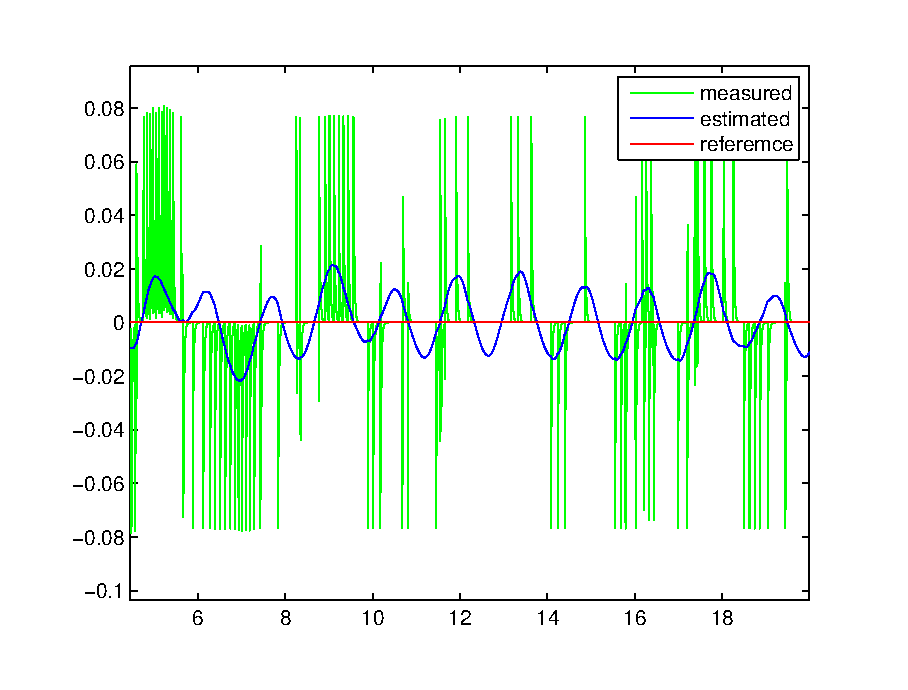
\includegraphics[width=0.9\linewidth]{Part4_pictures/p4p2_noint/riktig_Q/elevationRate_PDreg_P1.eps} 
    \caption{Elevation rate}
    \label{fig:p4p2nointP4e}
\end{subfigure}
\begin{subfigure}{0.5\textwidth}
    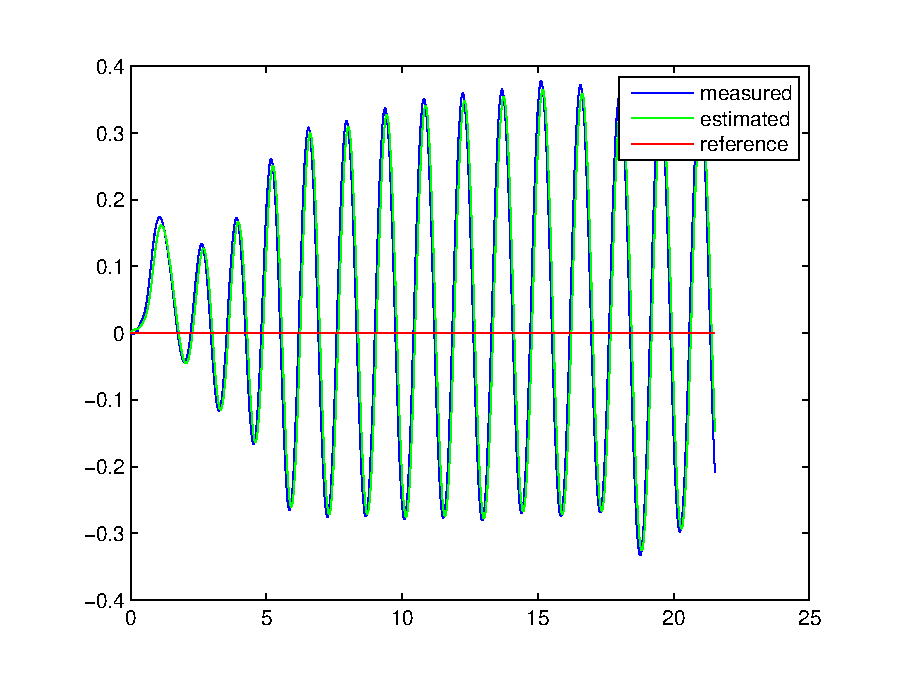
\includegraphics[width=0.9\linewidth]{Part4_pictures/p4p2_noint/riktig_Q/pich_PDreg_P1.eps}
    \caption{Pitch angle}
    \label{fig:p4p2nointP4p}
\end{subfigure}
\caption{Showing an oscillating response with no damping over time. r = 5, $\alpha = \frac{\pi}{50}$ and $\theta = \frac{\pi}{15}$. Q = [150 10 250]}
\label{p4p2nointP4}
\end{figure}

\subsubsection{With integral effect}
\begin{figure}[H]
\graphicspath{ {Part4_pictures/}}
\begin{subfigure}{0.5\textwidth}
    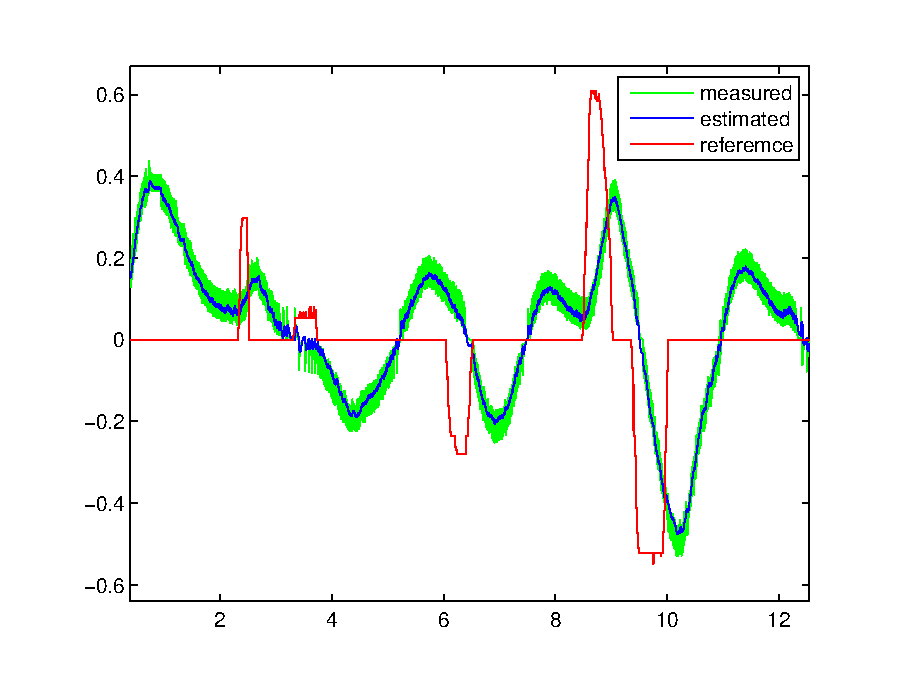
\includegraphics[width=0.9\linewidth]{Part4_pictures/p4p2_int/p1_elevrate.eps} 
    \caption{Elevation rate}
    \label{fig:p4p2intP1e}
\end{subfigure}
\begin{subfigure}{0.5\textwidth}
    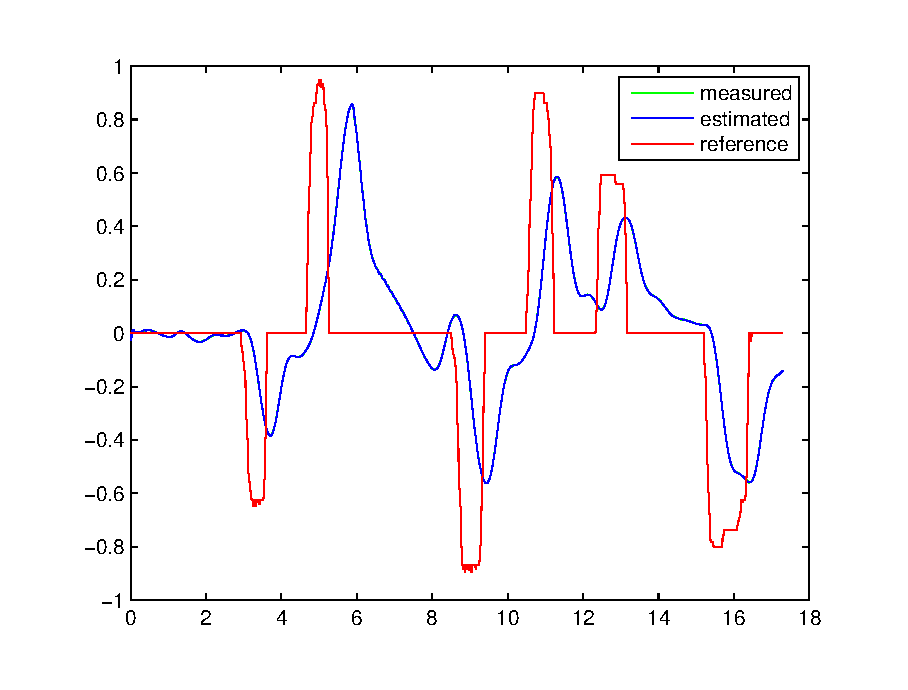
\includegraphics[width=0.9\linewidth]{Part4_pictures/p4p2_int/p1_pitch.eps}
    \caption{Pitch angle}
    \label{fig:p4p2intP1p}
\end{subfigure}
\caption{Same poles as used without integral effect $\alpha = \frac{\pi}{80}$, $\theta = \frac{\pi}{15}$ and r = 50. Q = [50 10 250 50 140]}
\label{p4p2intP1}
\end{figure}

\begin{figure}[H]
\graphicspath{ {Part4_pictures/}}
\begin{subfigure}{0.5\textwidth}
    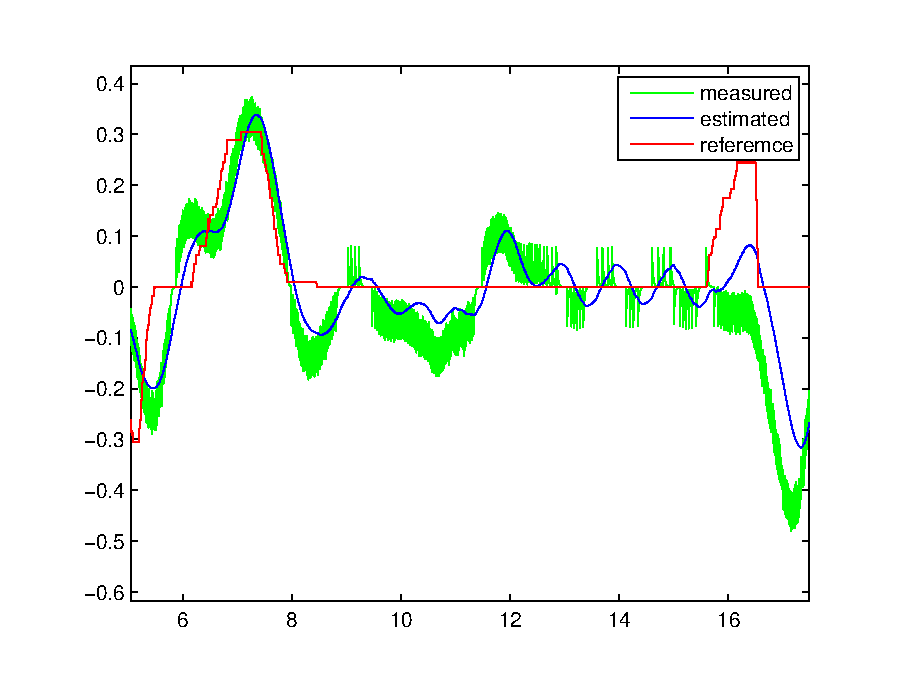
\includegraphics[width=0.9\linewidth]{Part4_pictures/p4p2_int/PID_reg_p8_elevation.eps} 
    \caption{Elevation rate}
    \label{fig:p4p2intP6e}
\end{subfigure}
\begin{subfigure}{0.5\textwidth}
    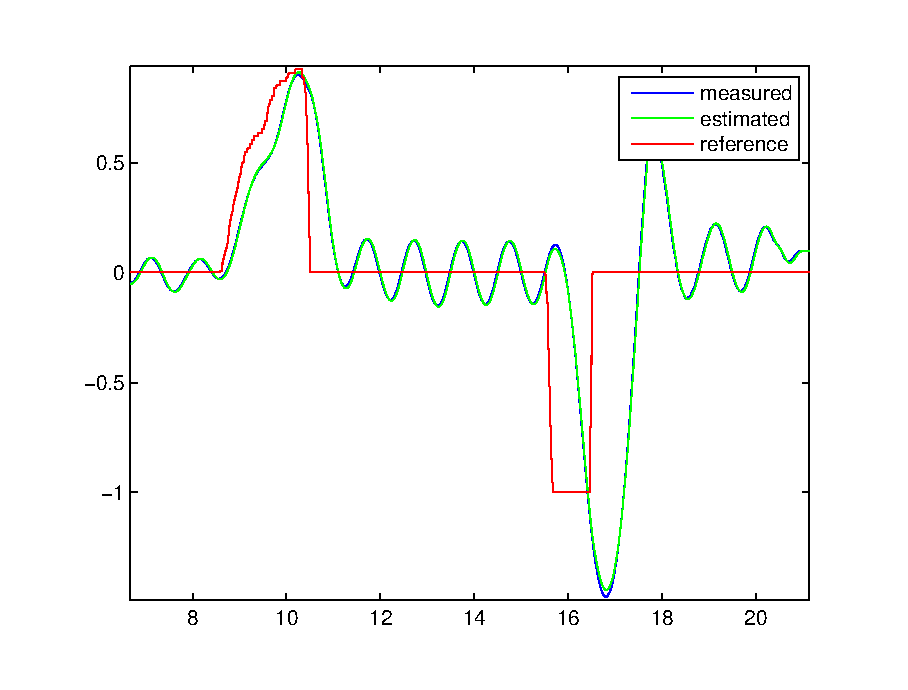
\includegraphics[width=0.9\linewidth]{Part4_pictures/p4p2_int/PID_reg_p8_pitch.eps}
    \caption{Pitch angle}
    \label{fig:p4p2intP6p}
\end{subfigure}
\caption{Using only real poles. Q = [50 10 250 50 140]}
\label{p4p2intP6}
\end{figure}
\newpage

\section{Nomenclature}%%%%%%%%%%%%%%%%%%%%%%%%%%%%%%%%%%%%%%%%%%%%%%%%%%%%%%%%%%%%%%%%%%%%%%%

\begin{center}
\begin{tabular}{ l  c  l }{Tabel 1}\\
  \hline			
    e & - & elevation angle [rad]\\
    $\tilde{e}$ & -& elevation angle (after coordinate transformation) [rad]\\
    $e{}^*$& - & linearization point elevation angle [rad]\\
    $\tilde{e}_c$ & - &reference for elevation [rad]\\
    $F_f$ &- & force generated by front propeller [N]\\
    $F_b$ &- & force generated back propeller [N]\\
    $F_{g,b}$ &- & gravitational force of back motor [N]\\
    $F_{g,c}$ & - & gravitational force of counterweight [N]\\
    $F_{g,f}$ & - & gravitational force of front motor [N]\\
    g & - & gravitational constant [$m/s^2$]\\
    J & - & cost function of linear quadratic regulator\\
    $J_e$ & - & moment of inertia about elevation axis [kg $m^2$]\\
    $J_p$ & - & moment of inertia about pitch axis [kg $m^2$] \\
    $J_\lambda$ & - & moment of inertia about travel axis [kg $m^2$]\\
    \textbf{K} & - & gain matrix of linear quadratic regulator\\
    $K_f$ & - & motor force constant [N/V]\\
    $K_{pd}$ &  - & controller gain [\(-\)] \\
    $K_{pp}$ & - & controller gain [\(-\)] \\
    $K_{rp}$ & - & controller gain [\(-\)] \\
    \textbf{L} & - & gain matrix of linear observer\\
    $l_c$ & - & distance from elevation axis to counterweight [m]\\
    $l_h$ & - & distance from elevation axis to helicopter head [m]\\
    $l_p$ & - & distance from pitch axis to motor [m]\\
    $m_p$ & - & motor mass [kg]\\
    $m_c$ & - & counterweight mass [kg]\\
  \hline  
\end{tabular}
\end{center}

\begin{center}
\begin{tabular}{ l  c  l }{Table 2}\\
  \hline			
    p &- &pitch angle [rad]\\
    \textbf{P}& -& gain matrix\\
    $\tilde{p}$&- &pitch angle (after coordinate transformation) [rad]\\
    $p{}^*$ &-& linearization point pitch angle [rad]\\
    $\tilde{p}_c$ &-& reference for pitch [rad]\\
    \textbf{Q}& -& weighting matrix of linear quadratic regulator\\
    \textbf{r} & - & reference vector\\
    \textbf{R}& -& weighting matrix of linear quadratic regulator\\
    t &- &time [s]\\
    \textbf{u}& - &input vector\\
    $V_b$ &- &voltage back motor [V]\\
    $V_d$ &- &voltage difference, $V_f - V_b$ [V]\\
    $\tilde{V}_d$ &- &voltage difference (after coordinate transformation) [V]\\
    $V_{d}^*$& - &linearization point voltage difference [V]\\
    $V_f$ &- &voltage front motor [V]\\
    $V_s$ &- &voltage sum, $V_f + V_b$ [V]\\
    $\tilde{V}_s$&-& voltage sum (after coordinate transformation) [V]\\
    $V_{s}^*$ &- &linearization point voltage sum [V]\\
    \textbf{x} &- &state vector\\
    \textbf{y}& - &output vector\\
    $\lambda$ &- &travel angle [rad]\\
    $\tilde{\lambda}$ &- &travel angle (after coordinate transformation) [rad]\\
    $\lambda{}^*$ &- &linearization point travel angle [rad]\\
    $\dot{\tilde{\lambda}}_c$& - &reference for travel rate [rad/s]\\
  \hline  
\end{tabular}
\end{center}